\documentclass[]{beamer}
%\usepackage[utopia]{mathdesign}
%\usepackage[no-math]{fontspec}
%\setmainfont{Liberation Serif}

\usepackage{minted}
% \usepackage{redhat}
\usepackage{hyperref}
\usepackage{ccicons}
\usepackage{ulem}

\usepackage{tikz}
\usetikzlibrary{arrows,shapes,snakes,automata,backgrounds,petri}

%gets rid of bottom navigation bars
\setbeamertemplate{footline}[frame number]{}

%gets rid of navigation symbols
\setbeamertemplate{navigation symbols}{}

\usepackage[export]{adjustbox}

\newcommand{\done}{\textcolor{teal}{\checkmark}}
\newcommand{\pull}[3]{\href{https://github.com/systemd/#1/pulls/#2}{#3 (\##2)}}
\newcommand{\pulldone}[3]{\pull{#1}{#2}{#3} \done}
\newcommand{\commit}[3]{\href{https://github.com/systemd/#1/commit/#2}{#3 (#2)}}
\newcommand{\commitdone}[3]{\commit{#1}{#2}{#3} \done}
%\newcommand\pp\pause
\newcommand\pp{}


\title{\textsc{Unifying /usr/bin and /usr/sbin}\\
  {\small a.k.a.}\\
  UsrMove is not done until SbinMerge is done}
\author{Zbigniew Jędrzejewski-Szmek}
\institute{%
  
\includegraphics[width=0.4\textwidth]{images/Logo-redhat-color-375.png}\\
  \medskip
  \textit{zbyszek@in.waw.pl}\\
  \medskip
  \ccbysa
}
\date{\tiny Flock 2024, Rochester 8.8.2024}

\begin{document}

\setbeamertemplate{itemize items}[square]

\begin{frame}
  \titlepage % Print the title page as the first slide
\end{frame}

\begin{frame}
  \frametitle{4-way split}

  \pp

  \begin{center}
    \huge
    \begin{tabular}{c|c}
      \texttt{/bin} & \texttt{/usr/bin} \\
      \hline
      \texttt{/sbin} &  \texttt{/usr/sbin} \\
    \end{tabular}
  \end{center}
\end{frame}

\begin{frame}
  \frametitle{(Some) History}

  \pause
  1969 — \textsc{\small UNIX} is written for PDP-7\\
  \visible<2>{
    \hbox to 0pt{
      \vbox to 0pt{
        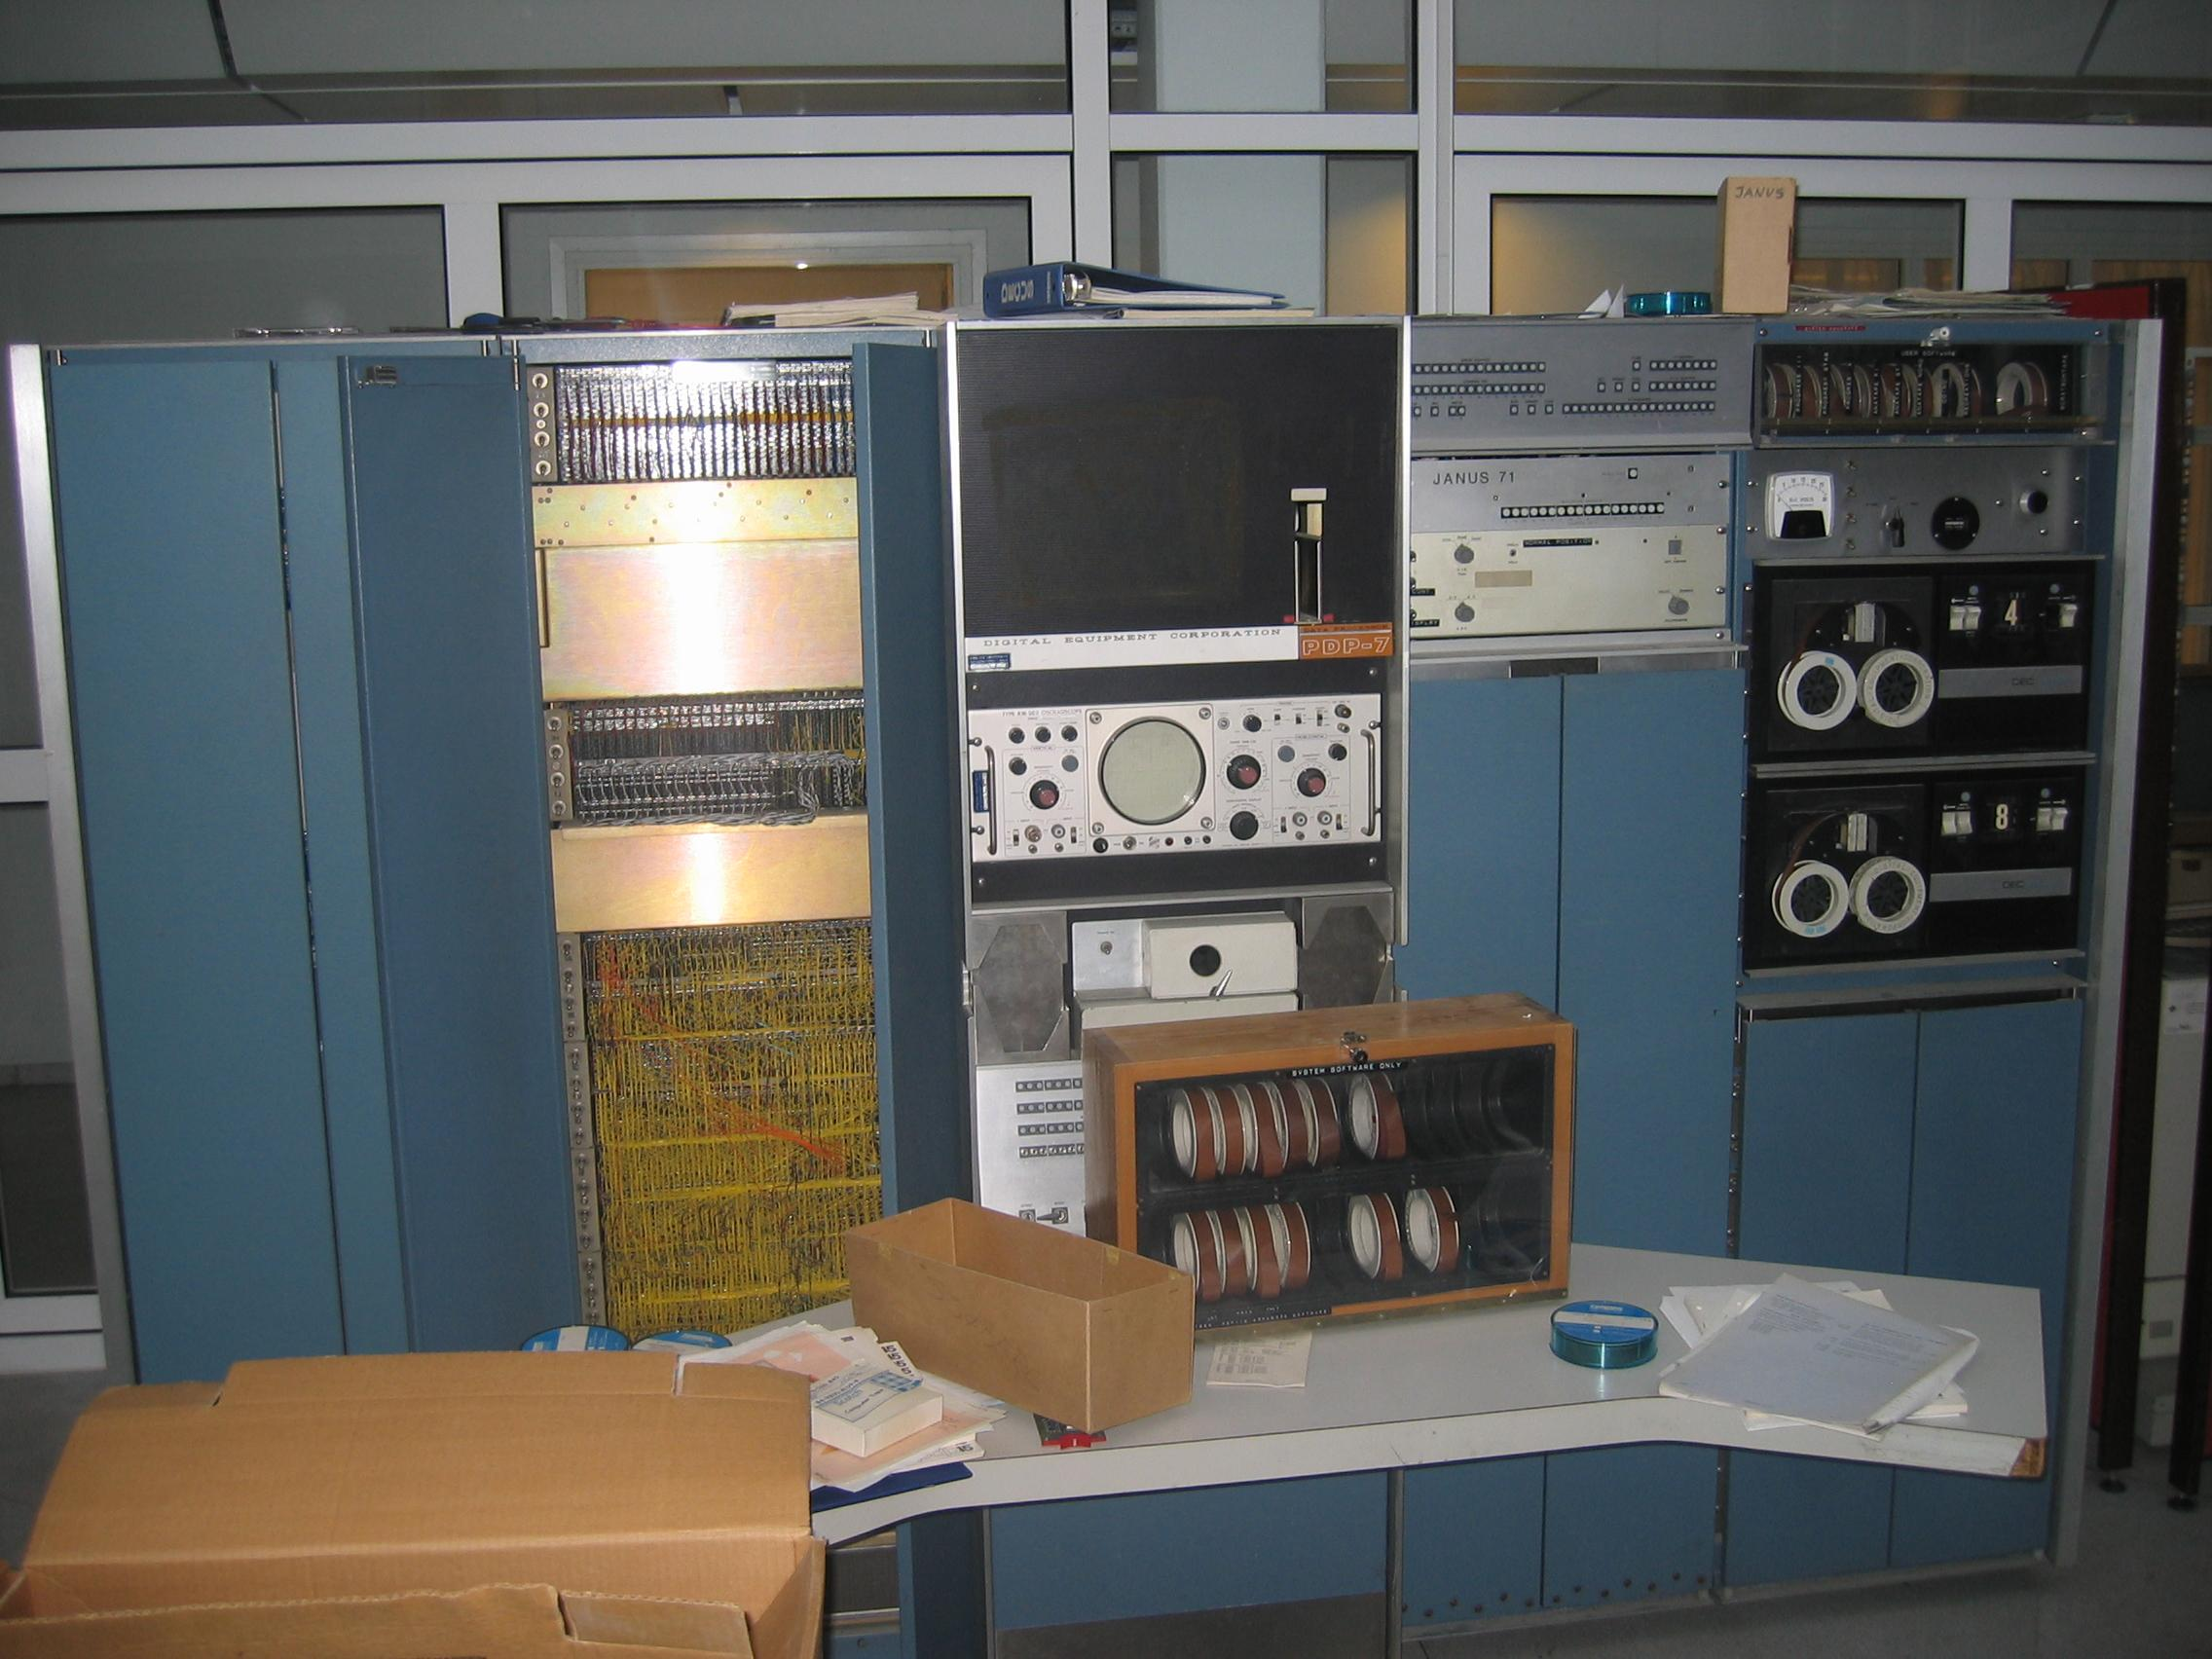
\includegraphics[width=0.8\textwidth,center]{images/Pdp-7-oslo-2004.jpeg}
      }
    }
    \hspace{-1em}
  }%
  \pause
  1971 — update for PDP-11 with two 1.5 MB disks\\
  \visible<3>{
    \hbox to 0pt{
      \vbox to 0pt{
        \includegraphics[width=0.8\textwidth,center]{images/pdp11-34-muzeumkomputerów.jpeg}\\
      }
    }
    \hspace{-1em}
  }%
  \pause
  \phantom{1670} — the OS "spills over" onto the second disk\\
  \phantom{1670 —} we have a four-way split\\
  \pause
  \phantom{1670} — a third disk is attached and /home is created\\
  \pause

  split \texttt{/usr} \textit{was} useful:\\
  \pause
  \phantom{1670} — fsck time proportional to fs size\\
  \phantom{1670} — periodic fsck (180 days or n mounts)\\
  \pause

  1990 — JFS in AIX 3.1\\
  1993 — NTFS in Windows NT\\
  2001 — EXT3 in Linux\\

  \pause
  initrds

  \vfill

  \tiny
  \url{http://lists.busybox.net/pipermail/busybox/2010-December/074114.html}\vspace{-5em}
\end{frame}

\begin{frame}
  \frametitle{Getting rid of separate /usr}

  \pause

  \href{https://systemd.io/THE_CASE_FOR_THE_USR_MERGE}{systemd/TheCaseForTheUsrMerge}\\

  \href{https://fedoraproject.org/wiki/Features/UsrMove}{Features/UsrMove} — Fedora 17 (2012)
\end{frame}

\begin{frame}
  \frametitle{Technical debt}

  \pause
  technical debt — \textit{the implied cost of future reworking required when
  choosing an easy but limited solution instead of a better approach
  that could take more time} [Wikipedia]\\
  \pause

  \hfill
  technical debt — \textit{something that made sense at the time, but now is
  just creating drag} [me]
\end{frame}

\begin{frame}
  \frametitle{Split \texttt{/bin} and \texttt{/sbin}}
  \framesubtitle{%
    … and \texttt{/usr/bin} and \texttt{/usr/sbin}\\
    … and \texttt{/usr/local/bin} and \texttt{/usr/local/sbin}}

  \pause
  \texttt{/sbin} — utilities used for system administration (and other root-only commands)
  [FHS]\\

  \pause
  example: \texttt{/sbin/mke2fs}\\

  \pause
  2006 — PolicyKit first commit\\
  polkit — allow unprivileged processes to elevate privileges via IPC
  \\

  \pause
  sudo

  \vfill

  \pause
  There are no ``root-only'' programs —\\
  \hspace*\fill separate /usr/sbin/ is now just technical debt too
\end{frame}

\begin{frame}
  \frametitle{Split \texttt{/bin} and \texttt{/sbin}}
  \framesubtitle{other reasons not to}

  \pause
  Different distributions do the split differently:\\
  {\tiny
  Fedora has \texttt{/sbin/ip}, Debian has \texttt{/bin/ip}\\
  Fedora has \texttt{/bin/chmem}, Debian has \texttt{/sbin/chmem}\\
  Fedora has \texttt{/bin/isosize}, Debian has \texttt{/sbin/isosize}\\
  Fedora has \texttt{/sbin/update-alternatives}, Debian has /bin\texttt{/update-alternatives}\\
  ...
  }
  \\

  \pause
  Also a problem for systemd unit files\\
  (\texttt{\small ExecStart=/usr/sbin/…})
  \\

  \pause
  \texttt{\$PATH} for all users includes both \texttt{/sbin} and \texttt{/bin}\\
  {\small (https://fedoraproject.org/wiki/Features/SbinSanity
  — Fedora 10, 2008)}
  \\

  \pause
  systemd sets clean environment for all services, with \texttt{/usr/sbin:/usr/bin}
  \small (09082a94b64f0b3b6cec44d4d8f423ab9abd1630, 2010)
\end{frame}

\begin{frame}
  \frametitle{Unifying \texttt{/usr/sbin} and \texttt{/usr/bin}}

  \pause
  Idea:~make \texttt{/usr/sbin} a symlink to \texttt{/usr/bin},\\
  \phantom{Idea:}~just like \texttt{/bin} is a symlink to \texttt{/usr/bin}\\

  \href{https://fedoraproject.org/wiki/Changes/Unify_bin_and_sbin}{Changes/Unify\_bin\_and\_sbin}
  — Fedora 41, 2024
\end{frame}

\begin{frame}
  \frametitle{Basic file system construction in Fedora}

  \pause
  \texttt{rpm.rpm} — the definitions of \texttt{\%\_bindir}, \texttt{\%\_sbindir}
  \\

  \pause
  \texttt{filesystem.rpm} — the actual layout on disk
  \\
\end{frame}

\begin{frame}
  \frametitle{The plan}
  \framesubtitle{Basic assumptions}

  \pause
  — normal packaging changes and scriptlets implement the move
  \\\pause

  — no "flag day"
  \\\pause
  \phantom{—} — conditional preparatory changes%, compatible with both worldviews
  \\\pause
  \phantom{—} — individual packages are updated when rebuilt
  \\\pause
  \phantom{—} — packages remain installable at all times
\end{frame}

\begin{frame}[fragile]
  \frametitle{The plan}
  % https://lists.fedoraproject.org/archives/list/devel@lists.fedoraproject.org/message/3562IKYYO4YLC5IPS3WSV3DNQXW3V7QG/

  \pause
  1. Remove Packaging Guidelines rule to use "historical" locations\\
     \hspace*{5em} for \texttt{/bin} vs. \texttt{/usr/bin}\\
     Remove Packaging Guidelines rule to use \texttt{/usr/sbin}
  \\

  \pause
  2. Adjust SELinux policy to make /sbin and /bin equivalent\\
  \textit{307 files changed, 862 insertions(+), 1261 deletions(-)}

  \hfill
\end{frame}

\begin{frame}[fragile]
  \frametitle{The plan}
  \framesubtitle{…ctd}

  3. Apply conditional fixes to packages:\\
  \textcolor{red}{FBTFS}:{\small
  \begin{minted}{spec}
  %install
  ln -s %{buildroot}%{_bindir}/foo \
        %{buildroot}%{_sbindir}/foo
  \end{minted}
  }
  and \textcolor{red}{FTI}:{\small
  \begin{minted}{spec}
  Transaction failed: Rpm transaction failed.
  - file /usr/sbin/sestatus conflicts between attempted
  installs of policycoreutils-3.6-5.fc41.x86_64
          and policycoreutils-3.6-5.fc41.x86_64
  - file /usr/sbin/named-checkzone conflicts between attempted
  installs of bind-utils-32:9.18.26-1.fc41.x86_64
          and bind-utils-32:9.18.26-1.fc41.x86_64
  \end{minted}
  }

  \hfill
\end{frame}

\begin{frame}[fragile]
  \frametitle{The plan}
  \framesubtitle{…ctd}

  4. Fix dependencies between packages:\\

   Package \texttt{a.rpm} has \mintinline{spec}|%files: %_sbindir/foo|\\
   Package \texttt{b.rpm} has \mintinline{spec}|Requires:/usr/sbin/foo|\\
   When rebuilt, \texttt{a.rpm} now has \texttt{/usr/bin/foo}, \texttt{b.rpm} FTI.
   \\\pause

   → Add compat \mintinline{spec}|Provides:/usr/sbin/foo|\\

   \texttt{a.rpm} adds:
  \begin{minted}{spec}
  %if "%_bindir" == "%_sbindir"
  Requires: filesystem(unmerged-sbin-symlinks)
  Provides: /usr/sbin/foo
  %endif
  \end{minted}

  \texttt{filesystem.rpm} will automatically create a symlink when a file is moved

  \hfill
\end{frame}

\begin{frame}[fragile]
  \frametitle{The plan}
  \framesubtitle{…ctd}

  5. Update \texttt{filesystem} and \texttt{rpm}\\
  Rebuild packages that would FTI\\
  (Some time later) Rebuild all other packages
   \\\pause

   \hfill

   <crash>

  \hfill

\end{frame}

\begin{frame}[fragile]
  \frametitle{What failed}

  \pause
  – Lorax\\
  "runtime-cleanup" phase to remove various executables by path
  %%   File were unexpectedly removed (/usr/bin/losetup, /usr/bin/mkswap)
  %%   and unexpectedly left behind
  %%   (62c2a714b7aa5c572795c22cb07696dffe3c2313,
  %%    https://src.fedoraproject.org/rpms/lorax-templates-rhel/pull-request/11)
  \\\pause

  — bootc/ostree/rpm-ostree\\
  filesystem.rpm is not used, custom fs layout
  % \\ {\small \url{https://gitlab.com/fedora/bootc/tracker/-/issues/29}}
  \\\pause

%%   Plan:
%%   - add Provides: filesystem(merged-sbin) in filesystem.rpm
%%     (https://src.fedoraproject.org/rpms/filesystem/pull-request/17)
%%   - conditionalize rpm-ostree to make /usr/sbin a symlink

  — Missing compat symlinks for paths \textit{not used} in \texttt{Requires}
%%   Package c.rpm has /usr/sbin/bar (%_sbindir/bar).
%%   After being rebuilt in the new world, it has /usr/bin/bar.
%%   Scripts and systemd unit files may use the old path.
%%   If new filesystem is installed, compat symlinks will be provided.
%%   But there is no explicit Requires on the new filesystem,
%%   so partially upgraded systems are broken.

%%   Plan:
%%   - add Provides:filesystem(merged-sbin) in filesystem.rpm
%%     (https://src.fedoraproject.org/rpms/filesystem/pull-request/17)
%%   - add an rpm fileattr generator to automatically add
%%     Requires:filesystem(merged-sbin)
%%     (https://src.fedoraproject.org/rpms/filesystem/pull-request/15)

%%   Package c.rpm will now pull in new fileystem.rpm, guaranteeing
%%   that /usr/sbin/bar and /usr/bin/bar both work.
\end{frame}

\begin{frame}[fragile]
  \frametitle{The plan (v2)}

  \pause
  5. Adjust Lorax, bootc/rpm-ostree, \texttt{filesystem}
  \\\pause

  6. (In rawhide, after f41 branching)\\
  Update \texttt{filesystem} and \texttt{rpm}\\
  Rebuild packages that would FTI\\
  (Some time later) Rebuild all other packages
  \\\pause

  7. filesystem.rpm will symlink \texttt{/usr/sbin} to \texttt{/usr/bin}\\
  if \texttt{/usr/sbin} only contains symlinks to \texttt{/usr/bin}
  \\\pause

  8. systemd will set \texttt{\$PATH} without \texttt{/usr/sbin}
  \\\pause

  The merge is complete: \texttt{/bin/foo}, \texttt{/sbin/foo}, and
  \texttt{/usr/sbin/foo} all point to \texttt{/usr/bin/foo}
\end{frame}

\begin{frame}
  \frametitle{Lessons}

  \pause
  — "Fedora Linux" is a complex ecosystem.\\
  \phantom{—} Many different actors, rpm content used in very different ways
  \\\pause
  — Change is hard
  \\\pause
  — Communication is important. The earlier the better
  \\\pause
  — Communication is not enough\\
  \phantom{—} Nobody anticipated problems with SELinux, Lorax, rpm-ostree…
  \\\pause
  — CI is great. OpenQA is great
  \\\pause
  — Lack of local CI is a problem\\
  \phantom{—} No realistic way to do a "trial run"
  \\\pause
  — Side-tags are great\\
  \phantom{—} (Revert changes in \texttt{filesystem} and \texttt{rpm}, dump side-tag)
  \\\pause
  — Big changes in Fedora are still possible, even if not easy
  \\\pause

  \vfill

  \hspace*{\fill}
  
\includegraphics[height=2em,width=2em]{images/Fedora_logo.png}
  
\includegraphics[height=2em,width=2em]{images/Fedora_logo.png}
  
\includegraphics[height=2em,width=2em]{images/Fedora_logo.png}
  
\includegraphics[height=2em,width=2em]{images/Fedora_logo.png}
  \hspace*{\fill}
\end{frame}

\end{document}
